\chapter{Estudo de caso: Perspectivas sobre o governo brasileiro}

\section{Introdução}

%Onde se motiva o estudo das eleições e fala pq tratará de colunas de jornalistas de notoriedade nacional. TUDO NESTE CAPÍTULO PRECISA SER BEM DIDÁTICO. FALAR DA FOLHA DILMAFACTSBYFOLHA

%mtos trabalhos de mineração de perspectiva tratam de discussão política. aproveitando o fato de que em 2010 se realizam as primeiras eleições para presidente realmente acompanhadas pela Internet, a gente decidiu fazer um estudo de caso neste assunto. Há outras pessoas pensando em coisas parecidas, como a galera do eleitorando, q criou o serviço pra fazer identificação de opinião em tweets. mas oq estamos propondo é fazer um estudo de análise das perspectivas contidas em blogs e colunas de jornalistas de notoriedade nacional, por eles serem muito lidos e contribuírem para a formação de opinião de seus leitores sobre o governo brasileiro, oq tem tudo a ver com a hora da urna.

Por ser um ano eleitoral, a

\section{Construção de corpus para estudo}

O corpus deste estudo é composto de artigos escritos para colunas de jornais e revistas ou para \emph{sites} sobre política. São textos de caráter eminentemente opinativo, que diferem de notícias tanto pela finalidade - \textbf{blibli} - quanto pela linguagem - \textbf{blabla}. Como o estudo visa à mineração das perspectivas pró/anti-governo federal, um critério básico para a escolha das colunas e \emph{sites} foi a existência de uma posição clara de crítica ou apoio ao atual governo. A notoriedade dos autores também foi considerada, facilitando a integração deste estudo a análises sobre a cobertura das Eleições 2010 em \textbf{TERMINE ISSO, e fale pq n políticos, e sim jornalistas}.

Este corpus, portanto, assim como outros revisados nesta monografia (vide capítulos \textbf{X} e \textbf{Y}), contém duas perspectivas em oposição sobre um mesmo assunto: o governo federal brasileiro. O lado pró-governo é composto de artigos veiculados em:

\begin{enumerate}

\item \textbf{Luis Nassif Online}\footnote{http://www.advivo.com.br/luisnassif/} Este é o \emph{blog} do jornalista Luis Nassif, premiado como Melhor Blog de Política pelo iBest 2008 \cite{ibest}. Nassif, que já trabalhou na TV Cultura e Rede Bandeirantes, mantém o \emph{blog} há cinco anos, enfocando principalmente assuntos relativos à política brasileira. Artigos do \emph{blog} são frequentemente citados, de forma positiva, em veículos de campanha pró-governo, como os \emph{sites} Blog da Dilma 13 Presidente\footnote{http://dilma13.blogspot.com/} e Os Amigos do Presidente Lula\footnote{http://osamigosdopresidentelula.blogspot.com/}. De fato, o Luis Nassif Online adota um posicionamento pró-governo, como comprovam os trechos a seguir:

\begin{quote}
\emph{"Desde o ano passado, estava claro [sic] a falta de competitividade de José Serra, seja por não ter feito um governo brilhante em São Paulo, por não representar o novo e por não conseguir desenvolver um discurso próprio."}

{\small Retirado de \emph{"Em Minas, a mãe de todas as batalhas"} - 02/09/2010} 
\end{quote}

\begin{quote}

\emph{"Na entrevista, Bonner se limitou a perguntar da dependência de Dilma em relação à Lula [...] A consequência foi Dilma rebatendo com facilidade cada bobagem dita, reforçando o discurso social, mas sem avançar em uma proposta sequer de programa, explicando a lógica das alianças políticas. E William Bonner interrompendo-a a toda hora, impedindo sequer uma resposta completa. Algo tão desastrado e mal educado que obrigou Fátima Bernardes, do alto de sua elegância, a calá-lo com um sinal, para que parasse de ser inconveniente."}

{ \small Retirado de \emph{"O dia em que William Bonner escorregou"} - 10/08/2010}

\end{quote}

Além de conter artigos escritos pelo próprio Luis Nassif, o \emph{blog} também publica textos de outros autores - alinhados, evidentemente, com os pontos de vista do jornalista.   

\item \textbf{Conversa Afiada}\footnote{http://www.conversaafiada.com.br/} O \emph{site} se define como um portal de jornalismo independente, contendo principalmente artigos produzidos por Paulo Henrique Amorim. O jornalista, que já trabalhou para as Redes Globo e Bandeirantes e para a revista Carta Capital, mantém o \emph{site} desde 2006. Enfocando a política brasileira, o Conversa Afiada apóia, dentre outras iniciativas do governo federal, a candidatura da ex-ministra Dilma Rousseff\footnote{http://www.conversaafiada.com.br/brasil/2010/07/02/mino-explica-por-que-apoia-a-dilma-porque-ela-e-melhor-que-o-serra/}. Os trechos abaixo justificam a escolha do \emph{site} como representante da mídia \emph{online} pró-governo:

\begin{quote}

\emph{"O Governo Lula é um sucesso e a popularidade dele, recordista desde o primeiro dia de Governo. Promoveu a inclusão social, ampliou a classe média e assistiu os pobres. Fez uma política externa que não tirou o sapato para os Estados Unidos. A Dilma é a sua legítima sucessora: foi a CEO do Governo Lula. O Serra é um nada."}

{\small Retirado de \emph{"A Dilma não é um tsunami. Dilma é o rio que segue para o mar"} - 27/08/2010}
\end{quote}

\begin{quote}

\emph{"Segundo a tevê DEMO-Tucana da Bahia, a afiliada da Globo, Jacques Wagner está na frente de Paulo Souto por 46\% a 19\%. Paulo Souto é o aliado de Serra na Bahia. A TV Bahia, também."}

{\small Retirado de \emph{"Sumiram com o dinheiro do Serra. Serra é barrado em procissão"} - 07/08/2010}
\end{quote}

Os artigos do \emph{site} muitas vezes citam notícias retiradas de portais, como o G1 ou UOL, a fim de contextualizar críticas e análises. 
% Prêmio iBest de Melhor Blog de Política, em eleição popular e da Academia iBest. 

\item \textbf{Escrevinhador}\footnote{http://www.rodrigovianna.com.br/} O \emph{blog}, mantido pelo \emph{site} da revista Caros Amigos, é escrito pelo jornalista Rodrigo Vianna, que também é repórter da Rede Record. Ele está no ar desde 2008, enfocando acontecimentos da vida política do Brasil e do Mundo. No que diz respeito ao Brasil, o conteúdo do \emph{blog} assume uma perspectiva pró-governo, como ilustram os trechos abaixo:

\begin{quote}

\emph{"Abandonado pelos aliados do DEM e do PSDB, em queda nas pesquisas, Serra refugia-se na mídia. O candidato do PSDB virou isso: porta-voz dos interesses da velha mídia. Faz sentido. É quem, em última instância, sustenta a candidatura."}

{\small Retirado de \emph{"Serra, porta-voz da velha mídia; é Zé ou Mané?"} - 19/08/2010}
\end{quote}

\begin{quote}
\emph{"O programa da Dilma foi um show. [...] Foi um programa em que Lula não apareceu mais que Dilma, e nem sumiu – porque seria falso, ela é a candidata dele. Foi um programa em que Lula passou o bastão a Dilma. De forma eficiente, corajosa e, ao mesmo tempo, emocionante."}

{\small Retirado de \emph{"Dilma acerta a mão; Serra quer virar 'Zé'"} - 18/08/2010}

\end{quote}

\item \textbf{Brasília, eu vi}\footnote{http://brasiliaeuvi.wordpress.com/} O \emph{blog}, escrito pelo jornalista Leandro Fortes, que também trabalha para a revista Carta Capital, agrega alguns de seus artigos para a revista e outros textos sobre política. Estes artigos têm boa recepção em \emph{sites} de campanha pró-governo, como o Blog da Dilma 13 Presidente\footnote{http://dilma13.blogspot.com/2010/08/caso-lunus-verdade-dos-fatos.html}. De fato, eles assumem uma perspectiva de defesa da situação, como justificam os trechos abaixo:


\begin{quote}
\emph{"Assim, enquanto a imprensa mundial se dedica a decodificar as engrenagens e circunstâncias que fizeram de Lula o mais importante líder mundial desse final de década, a imprensa brasileira se debate em como destituí-lo de toda glória, de reduzí-lo a um analfabeto funcional premiado pela sorte, a um manipulador de massas movido por programas de bolsas e incentivos [...]."}

{\small Retirado de \emph{"Não verás Lula nenhum"} - 18/05/2010}
\end{quote}

\begin{quote}

\emph{"Ao acusar o presidente Luiz Inácio Lula da Silva de ter transformado o Brasil em uma “república sindicalista”, José Serra optou por agregar a seu modelito eleitoral, definitivamente, o discurso udenista de origem, de forma literal, da maneira como foi concebido pelas elites brasileiras antes do golpe militar de 1964."}

{\small Retirado de \emph{"Serra precisa de mais amigos"} - 15/07/2010}
\end{quote}
\end{enumerate}


O lado anti-governo, por sua vez, é composto de artigos veiculados em:

\begin{enumerate}

\item \textbf{Reinaldo Azevedo}\footnote{http://veja.abril.com.br/blog/reinaldo/} O \emph{blog}, escrito pelo jornalista homônimo, é mantido pela revista Veja. Autor da frase \emph{"Tudo que é bom para o PT é ruim para o Brasil"} \cite{bom-pt-mau-brasil}, Reinaldo Azevedo, que já foi editor da Folha de S. Paulo, alimenta seu \emph{blog} com críticas ao governo atual, como evidenciam os trechos abaixo:

\begin{quote}

\emph{"O problema dos petistas é que eles são viciados no aulicismo, na cortesania. Ao conviver com pessoas que sempre têm um preço, ficam chocados e tomam como ofensa pessoal a descoberta de que nem todos se comportam com essa moral anã."}

{\small Retirado de \emph{"Presidente do PT repete ladainha autoritária do programa 'Rubriquei, mas não traguei'. Ou: 'Ai que vontade de censurar a Veja!!!' Contenha a coceira, companheiro!} - 15/07/2010} 
\end{quote}

\begin{quote}

\emph{"Cinco centrais sindicais assinaram um vergonhoso manifesto contra a candidatura do tucano José Serra à Presidência. Antes de mais nada, e a despeito da mentira essencial que está contida no texto — já falo a respeito —, cumpre destacar: trata-se de um manifesto ilegal, de mais um crime eleitoral escancarado."}

{\small Retirado de \emph{"Acuado pelo 'Rubriquei, mas não traguei', PT mobiliza centrais sindicais. E elas assinam um documento ilegal e mentiroso."} - 12/07/2010 }

\end{quote}

\item \textbf{Coluna do Augusto Nunes}\footnote{http://veja.abril.com.br/blog/augusto-nunes/} A coluna, parte da revista Veja, é escrita pelo jornalista Augusto Nunes, que também apresenta o programa Roda Viva na TV Cultura. Seus artigos têm má recepção em alguns veículos que defendem ou fazem campanha para o atual governo, como o Luis Nassif Online \cite{nassif-nunes} e o Blog da Dilma 13 Presidente \cite{dilma13-nunes}, justamente por assumirem uma posição anti-governo. Os trechos abaixo justificam esta perspectiva:


\begin{quote}

\emph{"Como todo sinal de alarme, o som de um neurônio em ebulição é  perturbador, mas muito útil. Quem tem juízo entenderá que Dilma Rousseff não é uma candidata em campanha. É uma ameaça a caminho."}

{\small Retirado de \emph{"O som perturbador do neurônio em ebulição"} - 20/07/2010}

\end{quote}

\begin{quote}

\emph{"O eleitor merece saber se Lula recebeu uma herança maldita e reconstruiu o país, como repete há pelo menos seis anos, ou se resolveu valer-se de mentiras e fantasias para desqualificar o legado do antecessor que acabou com a inflação, consolidou a democracia constitucional e fixou diretrizes econômicas que, em sua essência, vigoram até hoje."}

{\small Retirado de \emph{"FHC aceita o convite para o duelo que Lula não pode recusar."} - 11/02/2010}
\end{quote}

\item \textbf{Coluna do Diogo Mainardi}\footnote{http://veja.abril.com.br/blog/mainardi/} A coluna, escrita desde 2002, é a mais lida da revista Veja segundo ela mesma, reunindo críticas à política e à economia brasileiras. O jornalista Diogo Mainardi se opõe aos governos petistas, tendo inclusive publicado, em 2007, o livro Lula é Minha Anta \cite{lula-anta}, no qual agrupa diversos artigos escritos para sua coluna na Veja. Os trechos abaixo ilustram a posição de Mainardi como um grande crítico do governo do PT e de sua candidata Dilma Rousseff:

\begin{quote}

\emph{"Dilma Rousseff teve uma loja de produtos importados. O empreendimento durou menos de um ano e meio. Se Dilma Rousseff mostrar como presidente da República o mesmo talento que mostrou como empresária, o Brasil já pode ir fechando as portas."}

{\small Retirado de \emph{"Dilma 1,99 Rousseff"} - 04/09/2010}
\end{quote}  

\begin{quote}

\emph{"No futuro, quando alguém quiser relatar os fatos deste período, terá de recorrer necessariamente aos processos judiciais, que detalharam o modo lulista de se organizar, de se acumpliciar, de se infiltrar e de fazer negócios."}

{\small Retirado de \emph{"A história em inquéritos"} - 20/03/2010}
\end{quote}

\item \textbf{Portal de Carlos Alberto Sardenberg}\footnote{http://www.sardenberg.com.br/site/index.php} O portal contém artigos do jornalista para suas colunas nos jornais O Globo e O Estado de S. Paulo, além de outros textos de análise política e econômica. Além destas ocupações, Sardenberg também é comentarista da TV Globo e âncora da Rádio CBN, tecendo comentários sobre a economia mundial e brasileira. Os trechos abaixo transparecem seu posicionamento anti-governo: 

\begin{quote}

\emph{"O governo Lula não quer fazer concessões à iniciativa privada porque está num ímpeto estatizante, em ano eleitoral. Só que o Estado não tem os recursos para fazer nada de substancial. Fica por isso mesmo."}

{\small Retirado de \emph{"As tarefas de Lula"} - 22/03/2010}
\end{quote}

\begin{quote}

\emph{"É verdade que o país está de novo em um bom momento. Mas não é verdadeira a conclusão que o 'lulismo' tira disso: que isso tudo só está acontecendo porque Lula é o presidente."}

{\small Retirado de \emph{"A salvação?"} - 01/04/2010}
\end{quote}
\end{enumerate}

Todos os artigos contidos nesses veículos, publicados entre 01/01/2010 e 06/09/2010, foram coletados de forma automatizada com \emph{scripts} escritos nas linguagens de programação Python e UNIX Shell script. Todos eles estão disponíveis no repositório \emph{online} de Aline Bessa \cite{alibezz-github}. O período fixado, por fazer parte de um ano eleitoral, encerra uma quantidade significativa de artigos pró e anti-governo - muitos deles focados na sucessão presidencial. Por este motivo, e também para manter o escopo do estudo atrelado às Eleições 2010, artigos de anos anteriores não foram coletados. Como os jornalistas eventualmente também publicam sobre outros temas, foi feita uma filtragem nos artigos, de modo que só restaram aqueles que contêm pelo menos uma das seguintes palavras-chave: "Lula", "FHC", "Dilma", "Serra", "Marina", "PT", "PV", "PSDB". Todos os documentos foram, por fim, anonimizados, para que os nomes de seus autores não interferissem nos estudos. 

%Em seguida, para evitar ruído causado por textos muito pequenos, foram descartados do corpus todos os artigos com menos de 100 palavras. 
%A fim de diminuir as discrepâncias entre as quantidades de artigos extraídas, de modo que todos os veículos pudessem contribuir de forma significativa para o estudo, foram agregados ao corpus, em alguns casos, apenas artigos com um número de palavras maior ou igual a um determinado valor. Este valor foi escolhido empiricamente para cada veículo, mas isto não causa perda de generalidade no estudos quais foram escolhidos aleatoriamente. A Tabela \ref{tab1:estudo} indica quantos artigos, por veículo, estavam disponíveis em cada etapa da composição do corpus. Todos os programas desenvolvidos para todas as etapas estão disponíveis no repositório \emph{online} de Aline Bessa \cite{alibezz-github}.

\begin{table}[t]
\centering
\begin{tabular}{| l | l | p{5cm} | }
\hline

\textbf{Veículo} & \textbf{Coleta} & \textbf{Filtragem/Anonimização} \\ \hline

\textbf{Reinaldo Azevedo} & 2490 & 2377\ensuremath{^*} \\ \hline
\textbf{Augusto Nunes} & 579 & 450 \\ \hline
\textbf{Diogo Mainardi} & 40 & 32 \\ \hline
\textbf{Carlos Sardenberg} & 59 & 33  \\ \hline
\textbf{Conversa Afiada} & 375 & 337  \\ \hline
\textbf{Luis Nassif Online} & 994 & 525 \\ \hline
\textbf{Escrevinhador} & 222 & 179  \\ \hline
\textbf{Brasília, eu vi} & 34 & 24  \\ \hline
\end{tabular}
\label{tab1:estudo}
\caption{Quantidades de artigos disponíveis em cada etapa da construção do corpus. \ensuremath{^*}Apenas 550, amostrados aleatoriamente, foram aproveitados.}
\end{table}

Após filtragem e anonimização, restaram 1065 artigos pró-governo e 2747 anti-governo. Para os estudos feitos com o corpus, envolvendo o classificador Naïve Bayes e o modelo de tópicos L-LDA, reduziu-se a quantidade de documentos anti-governo para 1065, utilizando-se apenas 550 dos 2377 artigos extraídos do \emph{blog} de Reinaldo Azevedo, amostrados aleatoriamente. Essa estratégia foi adotada porque o desempenho do  Naïve Bayes se mostrou sensível a quantidades muito discrepantes de palavras por perspectiva. Como o uso do L-LDA estende as análises feitas com o classificador, decidiu-se manter o corpus idêntico para ambos os estudos. 

O número de artigos coletados em cada veículo varia bastante, como pode ser observado na Tabela \ref{tab1:estudo}. No corpus \textbf{Bitterlemons}\footnote{A descrição deste corpus encontra-se na seção \textbf{XXX} desta monografia.}, estudado por Lin et al., o número de artigos disponíveis também varia bastante de autor para autor, e os resultados obtidos são de alta qualidade \cite{lin-et-al2006}. Isto reforça a ideia de que essa variação não interfere significativamente na qualidade dos experimentos feitos com o corpus deste estudo de caso. É válido ressaltar, por fim, que os autores dos artigos muitas vezes colocam trechos de notícias, ou mesmo textos opinativos de outros autores, em seus artigos, colaborando para a riqueza da linguagem no corpus.%Os estudos de Mullen e Malouf com um fórum de discussão política também sugerem que a contribuição dos participantes é assimétrica, obedecendo a uma distribuição livre de escala

% Um estudo de Mullen e Malouf com um fórum de discussão política aponta, inclusive, que   % Isto é comum em outros corpora, como apontam os estudos de Mullen e Malouf com fóruns de discussão política%Os estudos de Tony Mullen e Robert Malouf com um fórum de discussão política dos Estados Unidos  \cite{malouf-taking_sides} \cite{aaai-politcs} %apenas 24 do \emph{blog} de Leandro Fortes foram aproveitados. 
%A escolha das percentagens foi empírica, visando a definir quantidades de artigos, para cada veículo, tão parecidas quanto possível - mas que, ao mesmo tempo, respeitassem as disponibilidades iniciais de artigos. Assim como a quantidade de arquivos do Luis Nassif Online é maior que a do Escrevinhador na etapa de \emph{download}, isto se conserva na etapa final da composição do corpus. Por ser uma heurística, cuja finalidade é simplesmente otimizar o aprendizado das perspectivas considerando veículos diferentes, não é necessário haver um rigor matemático na escolha destes valores. 

%Tem-se, portanto, um conjunto de artigos escritos sob duas perspectivas opostas: anti e pró governo federal. O número de artigos selecionados para cada perspectiva foi 499, de modo que o corpus possui 998 documentos. 

%foram, respectivamente, 499 e  Tem-se, respectivamente, Do primeiro lado, foram selecionados 499 textos; do segundo, 



% para o estudo. 

%  o que evidencia %A escolha do período deveu-se ao fato de que 2010, por ser ano eleitoral, concentra muitas opiniões a respeito do atual governo e seus possíveis sucessores à presidência,

%Para se traçar paralelos entre os resultados deste estudo e o comportamento da mídia tradicional brasileira, escolheu-se apenas artigos veiculados por jornalistas de notoriedade nacional

%os autores dos artigos são jornalistas de notoriedade nacional, o que confere ao estudo um caráter \textbf{bleble}.

% e notoriedade dos autores em nível nacional. 

%A seleção dos jornalistas levou em consideração dois fatores: o caráter opinativo de seus textos e a notoriedade em nível nacional.  


%Onde se fala dos critérios utilizados na escolha dos jornalistas (justifique com trechos e talz), download, tratamento de tags, período estudado, palavras-chave, número de caracteres. Idiossincrasias da coisa.


%Onde se explica detalhadamente as perspectivas do corpus, justifica-se o método, mostra-se o desempenho via 10-fold-cross-validation (fala pq escolheu essa também), discute-se questões de estilo e compara com o desempenho de outros artigos.

\section{Identificando perspectivas com um classificador Naïve Bayes}

O primeiro estudo conduzido com esse corpus consiste na classificação dos artigos de acordo com suas perspectivas - problema fundamental na área de Mineração de Perspectiva \cite{omsa}. O classificador Naïve Bayes, escolhido para o estudo por sua simplicidade, se mostrou adequado para o problema: a taxa de acerto obtida foi de 89.43\%; a precisão, de  89.68\%; a métrica F1, de 89.42\%. Assim como em outros artigos revisados para esta monografia \cite{lin-et-al2006} \cite{aaai-politics} \cite{klebanov}, esses valores foram obtidos via validação cruzada de dez dobras. O bom desempenho do método indica que a simples análise das palavras utilizadas nos artigos - desconsiderando, portanto, aspectos sintáticos e semânticos dos mesmos - já evidencia suas diferentes perspectivas. 

% e a avaliação das taxas de acerto, precisão e métrica F1 obtidas. 


% Se a taxa de acerto for alta, isto significa que a linguagem contida nos artigos, sem se considerar nenhum contexto, é suficiente para demarcar essas perspectivas. A fim de verificar esta hipótese, um classificador Naïve Bayes foi aplicado aos documentos.  A taxa de acerto obtida foi de 88.26\%; a precisão, de 89.47\%; e a métrica F1, de 88.16\%. 

%A taxa de acerto do classificador foi alta, comprovando a hipótese. 

Os valores obtidos com o classificador Naïve Bayes são comparáveis àqueles apresentados por Durant e Smith em seu trabalho sobre o posicionamento de \emph{blogs} frente às atitudes de George W. Bush na guerra do Iraque \cite{durant-smith}: 89.77\%. É válido ressaltar que, diferentemente da metodologia adotada por Durant e Smith, nenhuma palavra foi descartada no processamento dos textos para este estudo de caso. A alta taxa de acerto obtida encoraja estudos semelhantes ao desenvolvido por Durant e Smith, envolvendo \emph{blogs} e \emph{sites} políticos brasileiros escritos por cidadãos comuns. % Isto pode, inclusive, resultar em boas aplicações para análise automática de conteúdo.

Os artigos escolhidos para este corpus são compostos, muitas vezes, de textos de outros autores. Isto reforça o fato de que o classificador Naïve Bayes está efetivamente aprendendo as perspectivas dos documentos, em vez de estilos de escrita. De todo modo, assim como no estudo de Lin et al. com o corpus \textbf{Bitterlemons} \cite{lin-et-al2006}, foi conduzido um experimento em que os artigos pertencentes aos conjuntos de treinamento e teste são escritos por autores diferentes. Se o que está sendo aprendido são de fato as perspectivas dos documentos, a performance do classificador não deve ser muito diferente da obtida na validação cruzada de dez dobras. Testando com artigos da coluna de Augusto Nunes e do \emph{site} Conversa Afiada, e treinando com os demais, a taxa de acerto obtida foi de 92.79\%, acompanhada de precisão de 93.32\% e métrica F1 de 91.86\%. Este experimento, portanto, ratifica os outros resultados, evidenciando que o classificador Naïve Bayes cumpre bem a tarefa de identificar as perspectivas pró e anti governo.

% indicado para identificar perspectivas em artigos opinativos.
%Uma alta taxa de acerto também indica que a identificação de perspectiva política em \emph{blogs} brasileiros, cujas linguagens se assemelham às estudadas, pode apresentar um bom resultado.

%Se a taxa de acerto for alta, é possível pensar em aplicações que envolvam a identificação da perspectiva d


%- talvez até escritas por blogueiros comuns, em vez de jornalistas.


\section{Ilustrando a linguagem por perspectiva}
%Onde se explica o uso do L-LDA, o overlap de palavras, mostra-se snippets e talz.

%Com um modelo generativo L-LDA, é possível visualizar o uso de palavras por cada perspectiva do corpus.

%ESSE PAPO DE CONTAGEM TÁ MAIS COMPLICANDO DOQ AJUDANDO! MUDAR ESSE PAPO PARA 'ASSOCIOU MAIS FREQUENTEMENTE' por mim nem fala do estudo de lin et al., já justifica o método logo.
O bom desempenho do classificador Naïve Bayes indica que o simples processamento das palavras contidas nos artigos já é suficiente para a compreensão automática das perspectivas pró e anti governo. Para aprofundar o estudo sobre a linguagem de cada perspectiva, o modelo generativo L-LDA foi aplicado ao corpus \textbf{XYZ}. Cada artigo foi associado a dois tópicos: um genérico, igual para todos eles, e um referente à sua perspectiva (pró ou anti governo). Há, portanto, três tópicos diferentes nesta aplicação. O modelo relaciona as palavras contidas nos documentos a seus tópicos, de modo que aquelas mais comuns se associam mais frequentemente ao tópico genérico, enquanto outras, mais particulares de cada perspectiva, aos outros dois tópicos.   

%No estudo de Lin et al. com o corpus \textbf{Bitterlemons} \cite{lin-et-al2006}, utiliza-se as contagens de palavras geradas pelo classificador Naïve Bayes  Essas contagens \textbf{BLA}.  O uso do modelo L-LDA gera uma contagem de palavras mais flexível, por tópicos. Neste caso, assim como no capítulo \textbf{Freqs}, assume-se que cada artigo deste estudo se relaciona a dois tópicos:  Essa estratégia permite que palavras muito utilizadas por ambos os posicionamentos se associem mais fortemente ao tópico genérico, enquanto aquelas mais específicas se destaquem para os outros dois tópicos. As contagens geradas por um L-LDA, portanto, são mais direcionadas do que aquelas obtida com a simples contagem de todas as palavras por perspectiva.


% Diferentemente da simples contagem de todas as palavras por posicionamento, sugerida no estudo de Lin et al. com o corpus \textbf{Bitterlemons} \cite{lin-et-al2006}, o uso do L-LDA permite que cada documento possa se associar a mais de um tópico, adaptando as contagens para cada um deles.

\begin{table}[h]
\centering
\begin{tabular}{| l | p{10cm} | }
\hline
\textbf{Tópico} & \textbf{Palavras} \\ \hline
\textbf{Genérico} &  governo, brasil, serra, estado, lula, poder, presidente, nacional, vez, campanha, federal, história, pt, forma, pessoas, psdb, vida, brasileira, dinheiro, programa, texto, lei, ministro, nome, direito, brasileiro, momento, eleitoral, passado, ministério \\ \hline
\textbf{Pró-Governo} & serra, dilma, lula, psdb, presidente, pt, candidato, folha, tucano, eleições, partido, jornal, campanha, pesquisa, fhc, brasil, henrique, eleitoral, candidata, rousseff, globo, mundo, governador, entrevista, imprensa, presidência, petista, dem, candidatura, turno\\ \hline
\textbf{Anti-Governo} & dilma, lula, presidente, brasil, rousseff, pt, gente, candidata, mundo, candidato, petista, entrevista, partido, josé, eleições, chefe, tucano, presidência, sarney, eleitoral, petistas, fernando, casa, ministro, companheiro, amigo, planalto, brasileiros, senador, saber \\ \hline
\end{tabular}
\label{tab:palavras}
\caption{As trinta palavras mais frequentemente associadas aos tópicos Pró-Governo, Anti-Governo e Genérico, em ordem.}
\end{table}

%\textbf{BLABLABLA. Trinta. O tamanho das pal. é prop. ao número de vezes que cada uma delas se associou ao tópico X.}

A Tabela \ref{tab:palavras} indica que as palavras utilizadas por autores com posicionamentos diferentes muitas vezes são as mesmas, diferindo apenas na forma como são enfatizadas. Os artigos anti-governo, por exemplo, dão muito destaque às palavras \emph{lula} e \emph{dilma}; os pró-governo, por sua vez, também enfatizam estas palavras, mas dão um destaque maior a \emph{serra}, candidato à presidência pelo PSDB. A associação de palavras semelhantes, ainda que em intensidades diferentes, aos tópicos anti e pró governo advém do fato de que os artigos compartilham um tema geral - o governo brasileiro - e, consequentemente, o mesmo vocabulário básico. É diferente do que acontece quando os tópicos correspondem a temas diferentes em vez de perspectivas, como pode ser visto no trabalho de Ramage et al sobre L-LDA e \emph{tags} de \emph{blogs} \cite{llda}.

As palavras na Tabela \ref{tab:palavras} estão ordenadas de acordo com o número de vezes que se associam aos tópicos, mas isto não é suficiente para compreender o quanto cada perspectiva realmente as enfatiza. Visando a uma melhor compreensão do enfoque dado pelos diferentes pontos de vista do corpus, elas foram processadas pelo \emph{software} wordle\footnote{http://wordle.net}, resultando nas figuras \ref{situacao}, \ref{oposicao} e \ref{generico}. O tamanho das palavras nas imagens corresponde ao quanto elas se associam a cada tópico\footnote{Os valores correspondentes a cada uma das palavras, por tópico, se encontra no \textbf{ANEXO BLA}.}. As imagens \ref{situacao} e \ref{oposicao} evidenciam o destaque dado aos políticos Lula, Dilma Rousseff e José Serra nos artigos analisados. 


\begin{figure}[h!]
  \centering % este comando é usado para centralizar a Figura
  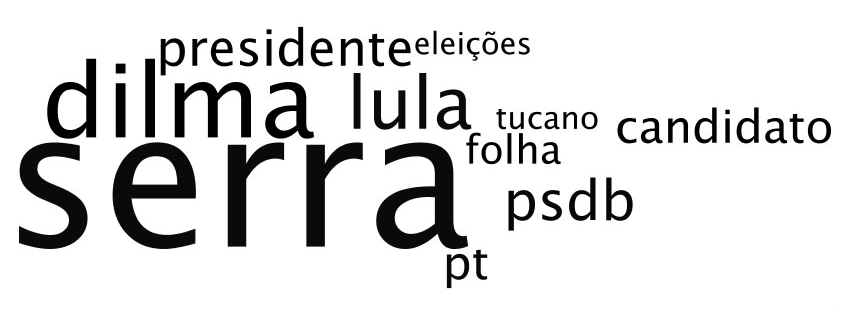
\includegraphics[width=12.5cm, height=6.5cm]{situacao.png}\\
  \caption{Representação gráfica para as trinta palavras mais frequentemente associadas ao tópico pró-governo.}
  \label{situacao}
\end{figure}

\begin{figure}[h!]
  \centering % este comando é usado para centralizar a Figura
  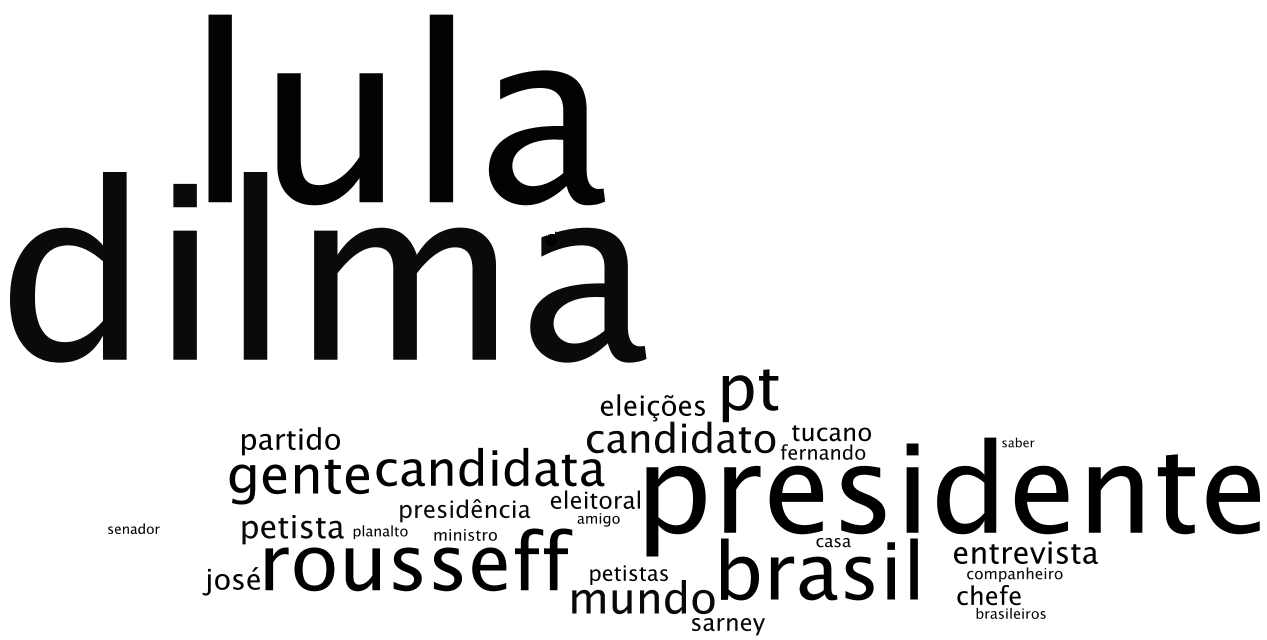
\includegraphics[width=12.5cm, height=6.5cm]{oposicao.png}\\
  \caption{Representação gráfica para as trinta palavras mais frequentemente associadas ao tópico anti-governo.}
  \label{oposicao}
\end{figure}

A imagem \ref{generico} dá certo destaque a Lula e José Serra, mas também enfatiza outros termos, como \emph{governo} e \emph{Brasil}, relacionados mais genericamente ao tema geral dos artigos: a política brasileira.

\begin{figure}[h!]
  \centering % este comando é usado para centralizar a Figura
  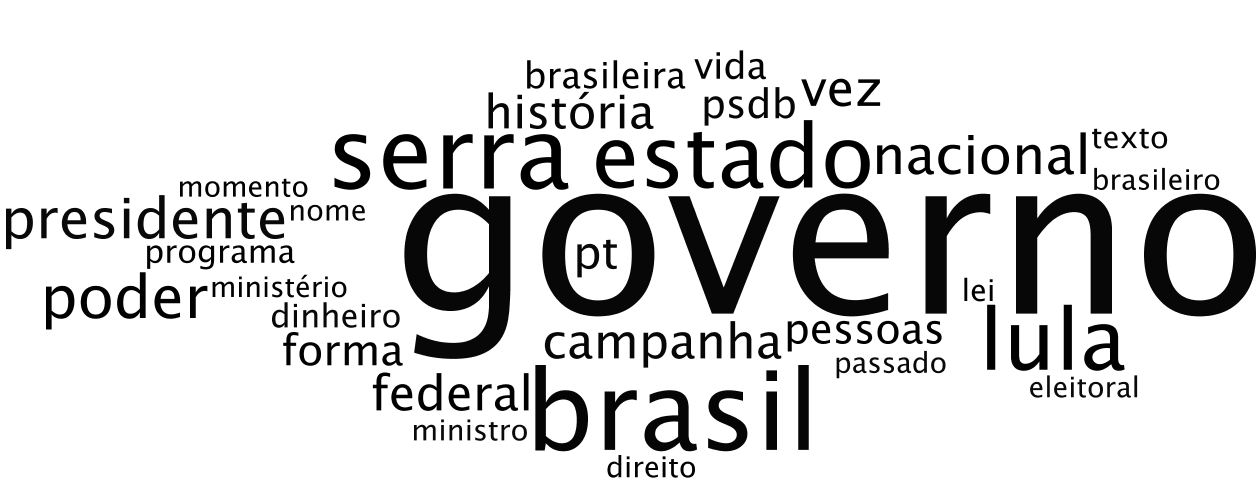
\includegraphics[width=12.5cm, height=6.5cm]{generico.png}\\
  \caption{Representação gráfica para as trinta palavras mais frequentemente associadas ao tópico genérico.}
  \label{generico}
\end{figure}


É válido ressaltar, por fim, que, apesar dos textos terem caráter opinativo, as palavras elencadas na Tabela \ref{tab:palavras} não carregam uma polaridade natural, como no caso dos adjetivos "bom" ou "ruim". Para aprofundar o entendimento da relação que elas estabelecem com as perspectivas dos artigos, portanto, recomenda-se ler um número razoável de passagens de texto que as contenham. Alguns trechos foram selecionados abaixo, em caráter ilustrativo:

\begin{quote}
\emph{"O que parece estarrecedor para quem nunca ouviu \textbf{Dilma} antes - e tenho colegas jornalistas que nunca a viram discursando ou dando \textbf{entrevista} - é absolutamente familiar para os frequentadores desta coluna. Que há nove meses têm acesso a veementes indícios, há muito transformados em provas documentais, de que \textbf{Dilma} é uma afronta imposta ao \textbf{Brasil} por \textbf{Lula}, num [sic] crime lesa-pátria sem perdão."}

{\small Retirado de "O som perturbador do neurônio em ebulição", da coluna de Augusto Nunes - 20/07/2010}
\end{quote}

\begin{quote}
\emph{"Que o \textbf{tucano} \textbf{José} Serra se saiu muito melhor no \textbf{Jornal} Nacional e que a eleição é, sim, de continuidade — no sentido de que não cabe mais falar em ruptura. E fiz uma crítica ou outra ao governo \textbf{Lula}."}

{\small Retirado de "A cabeça dos brasileiros... autoritários", do \emph{blog} de Reinaldo Azevedo - 15/08/2010}
\end{quote}

\begin{quote}

\emph{"A última bala na agulha do \textbf{Serra} é a baixaria. Só que, na era da internet, a baixaria – Lunus (para desconstruir Roseana Sarney) e aloprados do \textbf{PT} (para mandar as ambulâncias superfaturadas para o Inferno) – não tem o mesmo efeito do passado.É o caso dos aloprados do tal dossiê que ele vai ter que explicar na Justiça."}

{\small Retirado de "Serra só tem uma saída: pendurar FHC no pescoço", do \emph{site} Conversa Afiada - 07/06/2010}
\end{quote}

\begin{quote}
\emph{"A entrevista de \textbf{Dilma} ao JN foi didática: \textbf{Dilma} conseguiu colar sua \textbf{candidatura} como continuidade das políticas do governo \textbf{Lula}. Ponto pra ela.Por outro lado, o casal número um do JN da \textbf{Globo} escorregou e mostrou claramente contra quem trabalham em 2010 e a favor de quem se esforçam para mudar tudo o que está aí."}

{\small Retirado de "O povo não é (mais) bobo...", do \emph{blog} Luis Nassif Online - 10/08/2010}
\end{quote}




%ns \textbf{Bla e Ble} representam as palavras para os tópicos Pró-Governo e Anti-Governo

% a frequência de associação com cada um dos tópicos, mas esta informação não evidencia 
%constam abaixoOs trechos abaixo são passagens de alguns artigos contendo parte das palavras listadas para cada perspectiva. Eles sugerem que essas palavras funcionam como âncoras, a partir das quais os pontos de vista dos artigos são construídos. 

%ilustram pontos de vista associados a elas, aprofundando a compreensão 


%O modelo L-LDA provê um critério subjetivo para a melhor compreensão do bom desempenho obtido pelo classificador Naïve Bayes, evidenciando os diferentes enfoques encontrados no corpus. As imagens \textbf{BLA e BLI} facilitam a visualização das palavras listadas na Tabela \textbf{BLA}, para os tópicos pró-governo e anti-governo. O tamanho das palavras, nas imagens, é proporcional ao número de vezes que cada uma delas se associou a cada tópico. 

%É interessante observar como, de modo geral, as palavras da imagem \textbf{BLI} são menores do que aquelas contidas na imagem \textbf{BLA}. Isto sugere que o vocabulário dos artigos anti-governo é mais variado do que aquele empregado pelos pró-governo, de modo 

%A Tabela \ref{tab:palavras} contém as trinta palavras mais frequentemente associadas aos tópicos genérico, pró-governo e anti-governo. Elas estão ordenadas de acordo com a frequência da associação

%tanto termos relacionados à situação, como \emph{dilma} e \emph{lula} quanto outros associados à oposição, como \emph{serra} e \emph{psdb}. As palavras listadas para o tópico anti-governo m relação a todas as outras 28 palavras listadas. \textbf{A PALAVRA BLA, POR EXEMPLO, APARECE X VEZES MAIS QUE BLA NO LADO K...} IssoO que muda de uma perspectiva para outra neste caso, portanto, não são exatamente as palavras escolhidas, mas a forma como elas são enfatizadas. %falar de banner words, dizendo q existem mas oq realmente tem ajudado é a intensidade

% genéricocomum bem-estabelecido: a política brasileira. O que colabora para a identificação da perspectiva de um artigo com um Naïve Bayes, portanto, é o tratamento dado pelo mesmo a um determinado político ou acontecimento, evidenciado pelo uso mais ou menos intenso de determinadas palavras. 

%mostrar trechos dos textos

% de todos os artigos 

%A aplicação do L-LDA, diferentemente da simples contagem de palavras de todos os artigos de cada perspectiva,  em cada texto pela sua escalabilidade: é possível assumir que cada documento possui mais de um tópico, e segmentar as contagens de palavras de acordo com eles.


\section{Conclusões}

Onde se discute o que tudo isso quer dizer sobre nossa mídia, se fala um pouco da questão da linguística de corpus, como os jornais n necessariamente assumem um ponto de vista, mas contratam colunistas e talz. Amarrar questões futuras.

